\section{卷积神经网络}
\label{sec:cnn}

\begin{frame}
  \begin{center}
    \Huge{\textcolor{red}{卷积神经网络}}
  \end{center}

  \begin{enumerate}
    \item \alert{动机}
    \item \alert{卷积层}
    \item \alert{池化层}
    \item \alert{计算}    
  \end{enumerate}
\end{frame}

\subsection{动机}

\begin{frame}[fragile]{全连接网络}
  \begin{figure}
    \centering
    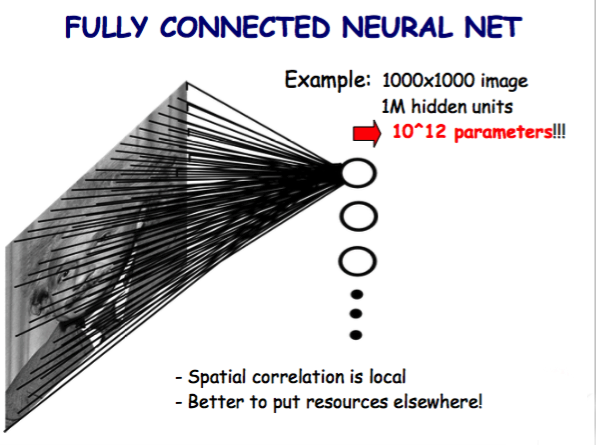
\includegraphics[width=0.8\textwidth]{conv-fcn.png}
  \end{figure}
\end{frame}

\begin{frame}[fragile]{局部连接网络}
  \begin{figure}
    \centering
    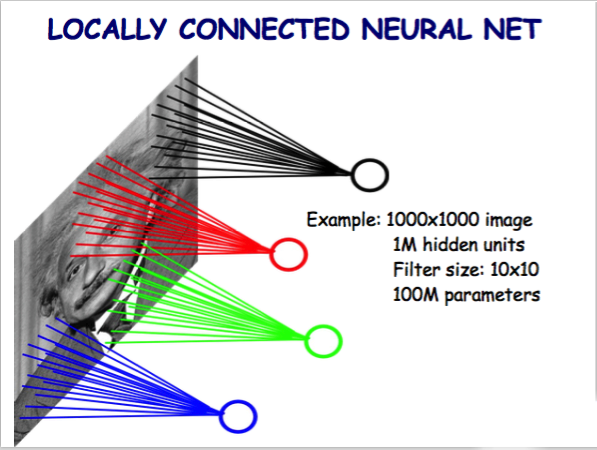
\includegraphics[width=0.8\textwidth]{conv-lcn.png}
  \end{figure}
\end{frame}

\begin{frame}[fragile]{权值共享:一个卷积核}
  \begin{figure}
    \centering
    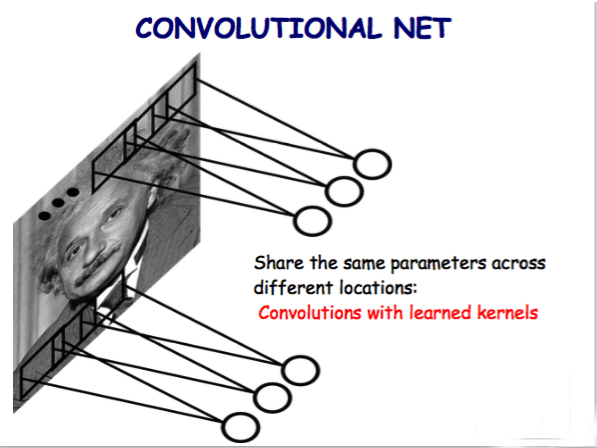
\includegraphics[width=0.8\textwidth]{conv-weight-shared.png}
  \end{figure}
\end{frame}

\begin{frame}[fragile]{权值共享:多个卷积核}
  \begin{figure}
    \centering
    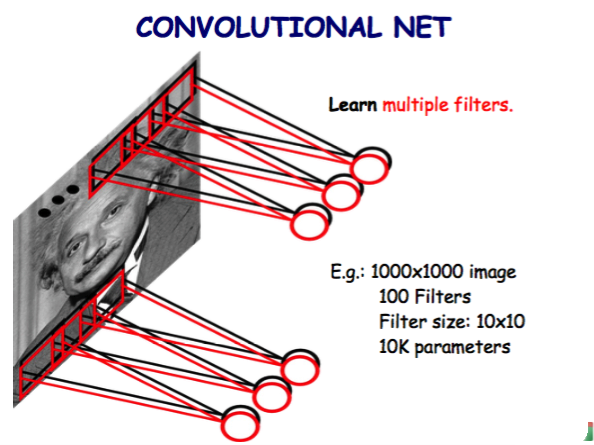
\includegraphics[width=0.8\textwidth]{conv-weight-shared-multi-filters.png}
  \end{figure}
\end{frame}

\subsection{架构模式}

\begin{frame}[fragile]{架构模式}
  \begin{figure}
    \centering
    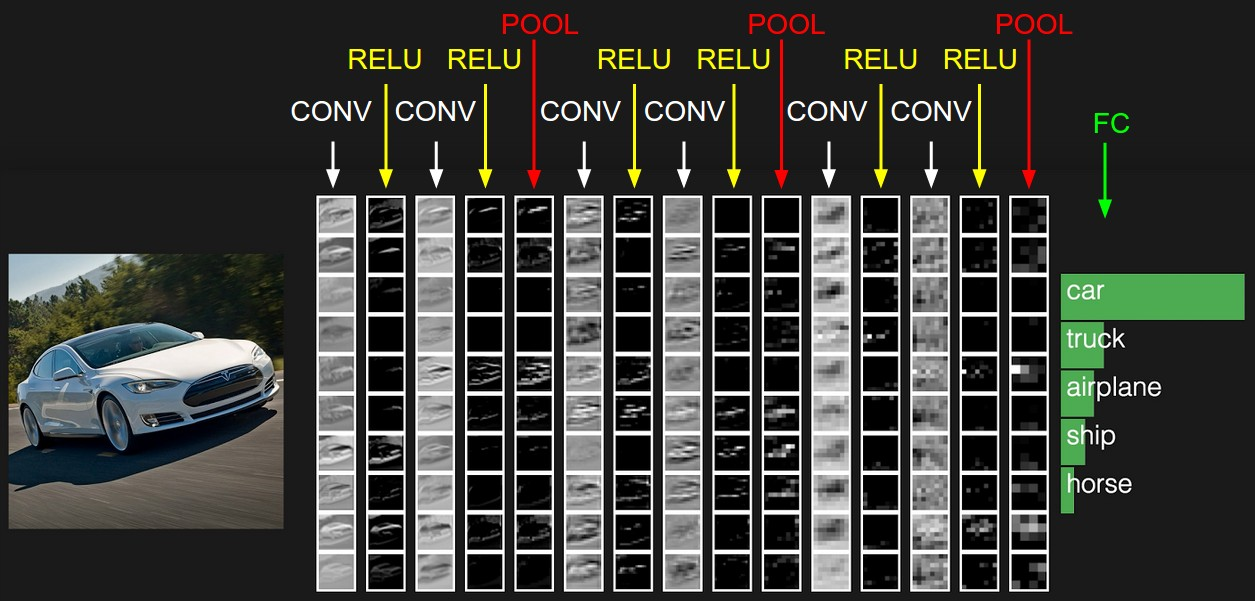
\includegraphics[width=0.8\textwidth]{conv-architecuture.jpeg}
  \end{figure}

  \begin{python}
INPUT -> [[CONV -> RELU]*N -> POOL?]*M -> [FC -> RELU]*K -> FC
  \end{python}  
\end{frame}

\subsection{卷积层}

\begin{frame}[fragile]{卷积运算}
  \begin{figure}
    \centering
    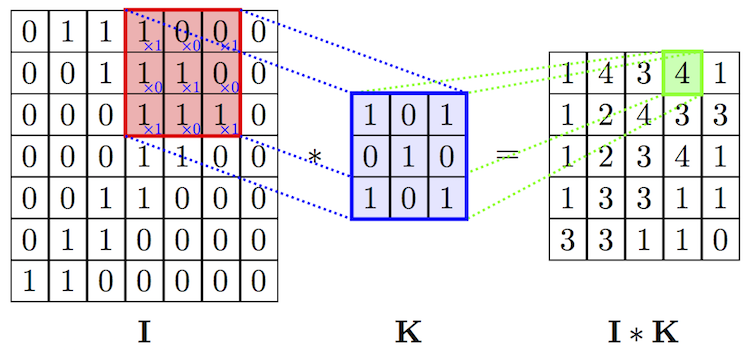
\includegraphics[width=0.8\textwidth]{conv-computation-1.png}
  \end{figure}
\end{frame}

\begin{frame}[fragile]{卷积运算}
  \begin{figure}
    \centering
    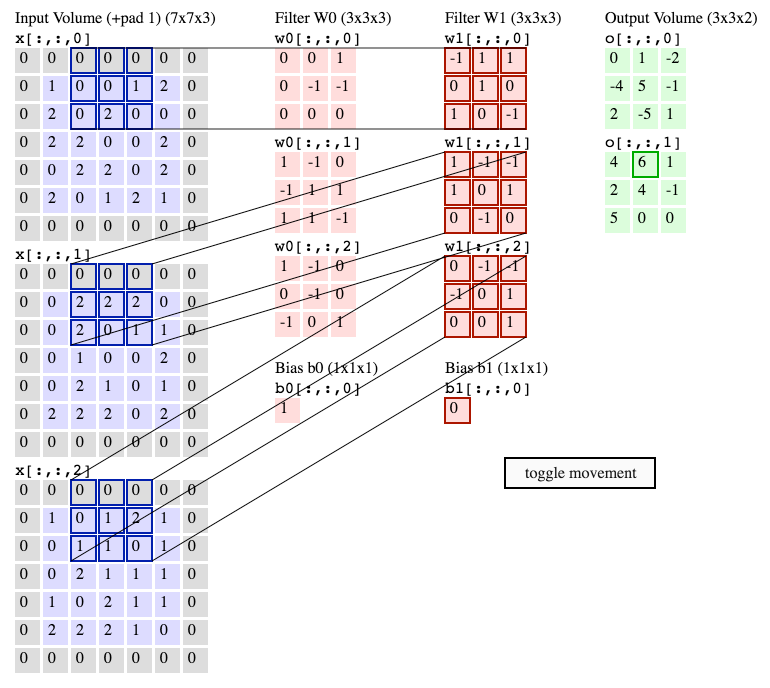
\includegraphics[width=0.65\textwidth]{convolutional-layer-6.png}
  \end{figure}
\end{frame}

\begin{frame}[fragile]{卷积运算}
  \begin{figure}
    \centering
    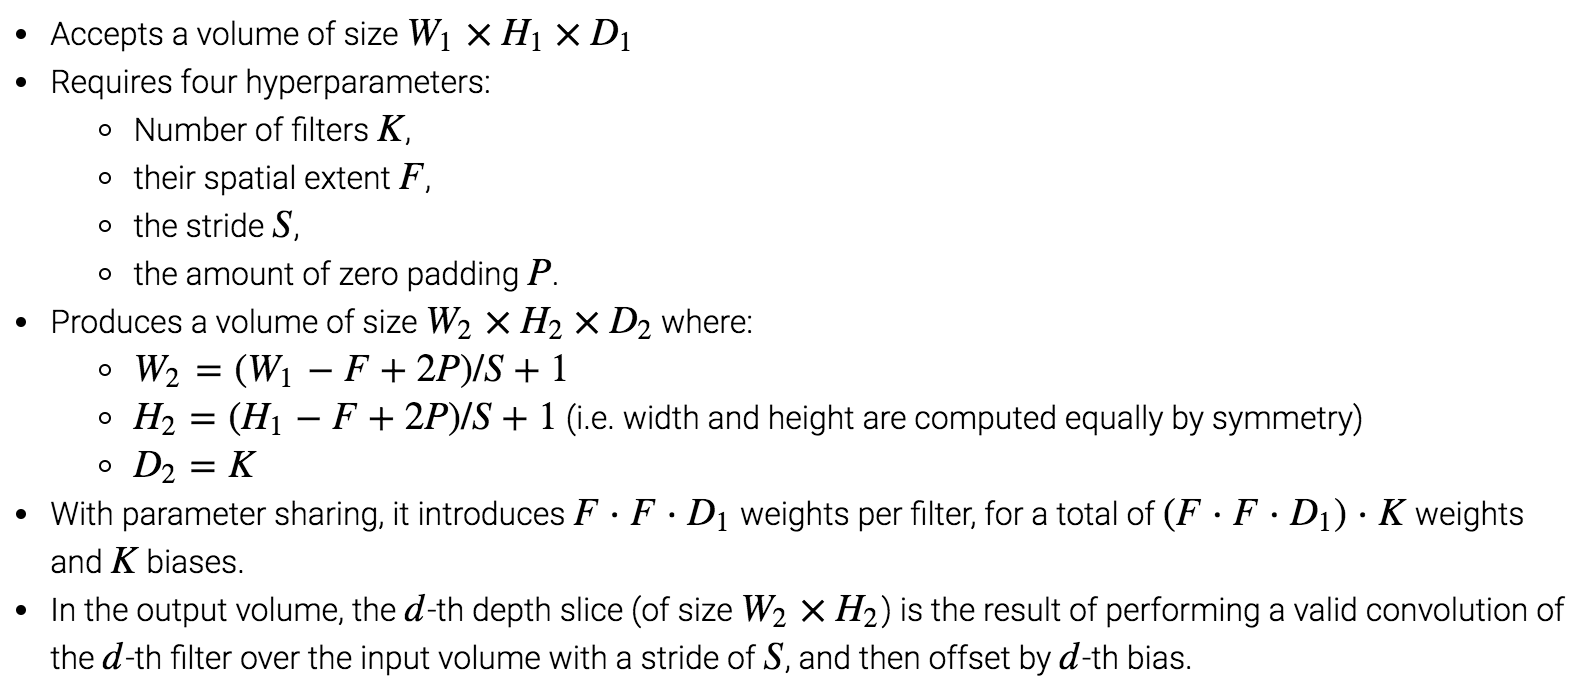
\includegraphics[width=0.65\textwidth]{conv-filter-computation.png}
  \end{figure}
\end{frame}

\begin{frame}[fragile]{卷积运算}
  \begin{figure}
    \centering
    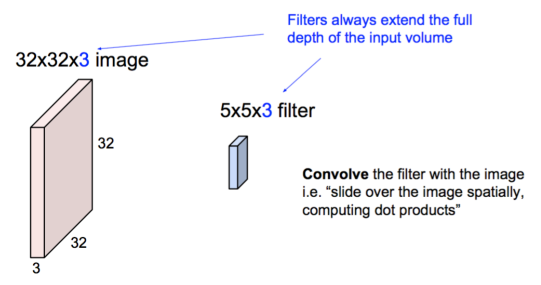
\includegraphics[width=0.8\textwidth]{convolutional-layer-1.png}
  \end{figure}
\end{frame}

\begin{frame}[fragile]{卷积运算}
  \begin{figure}
    \centering
    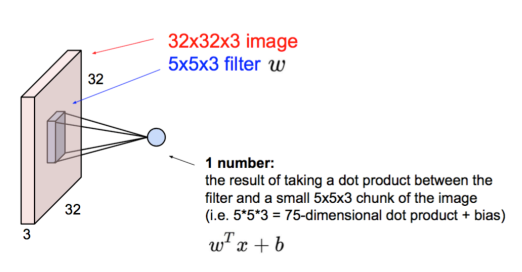
\includegraphics[width=0.8\textwidth]{convolutional-layer-2.png}
  \end{figure}
\end{frame}

\begin{frame}[fragile]{卷积运算}
  \begin{figure}
    \centering
    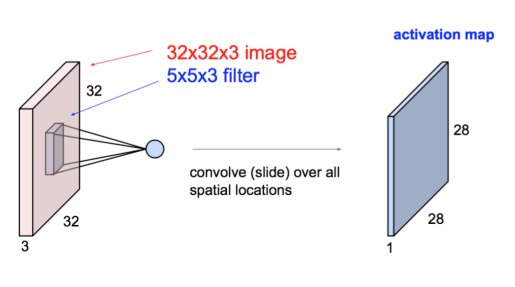
\includegraphics[width=0.8\textwidth]{convolutional-layer-3.png}
  \end{figure}
\end{frame}

\begin{frame}[fragile]{卷积运算}
  \begin{figure}
    \centering
    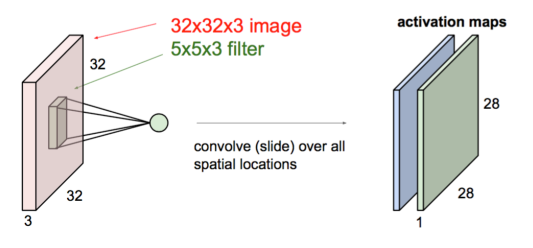
\includegraphics[width=0.8\textwidth]{convolutional-layer-4.png}
  \end{figure}
\end{frame}

\begin{frame}[fragile]{卷积运算}
  \begin{figure}
    \centering
    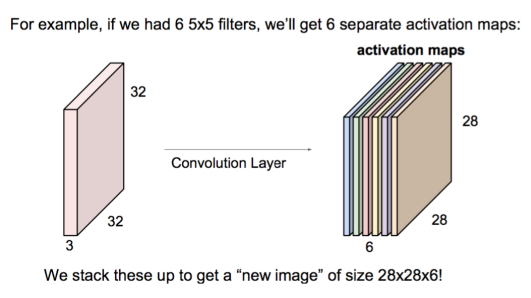
\includegraphics[width=0.8\textwidth]{convolutional-layer-5.png}
  \end{figure}
\end{frame}

\subsection{池化层}

\begin{frame}[fragile]{下采样:Max Pooling}
  \begin{figure}
    \centering
    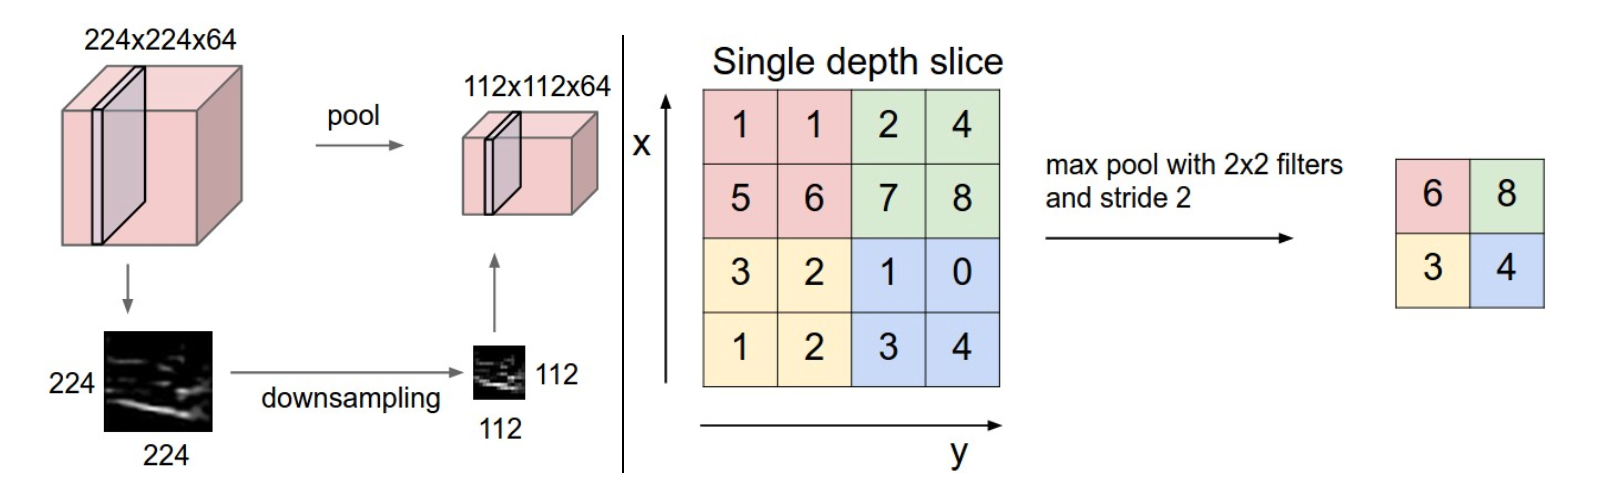
\includegraphics[width=0.8\textwidth]{conv-max-pooling.png}
  \end{figure}
\end{frame}

\begin{frame}[fragile]{下采样}
  \begin{figure}
    \centering
    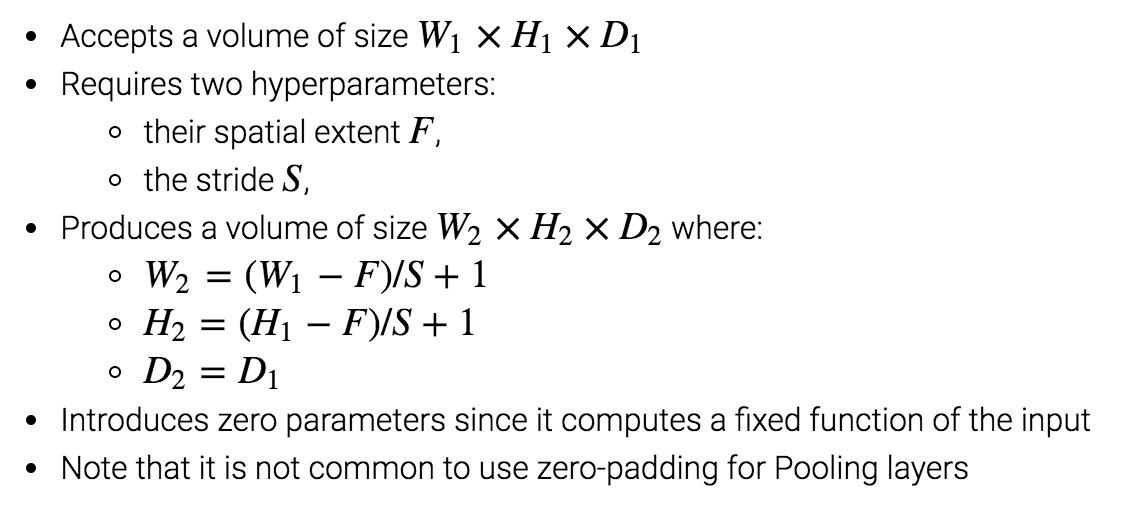
\includegraphics[width=0.8\textwidth]{conv-max-pooling-1.png}
  \end{figure}
\end{frame}

\subsection{计算}

\begin{frame}[fragile]{前向计算:卷积}
  \begin{figure}
    \centering
    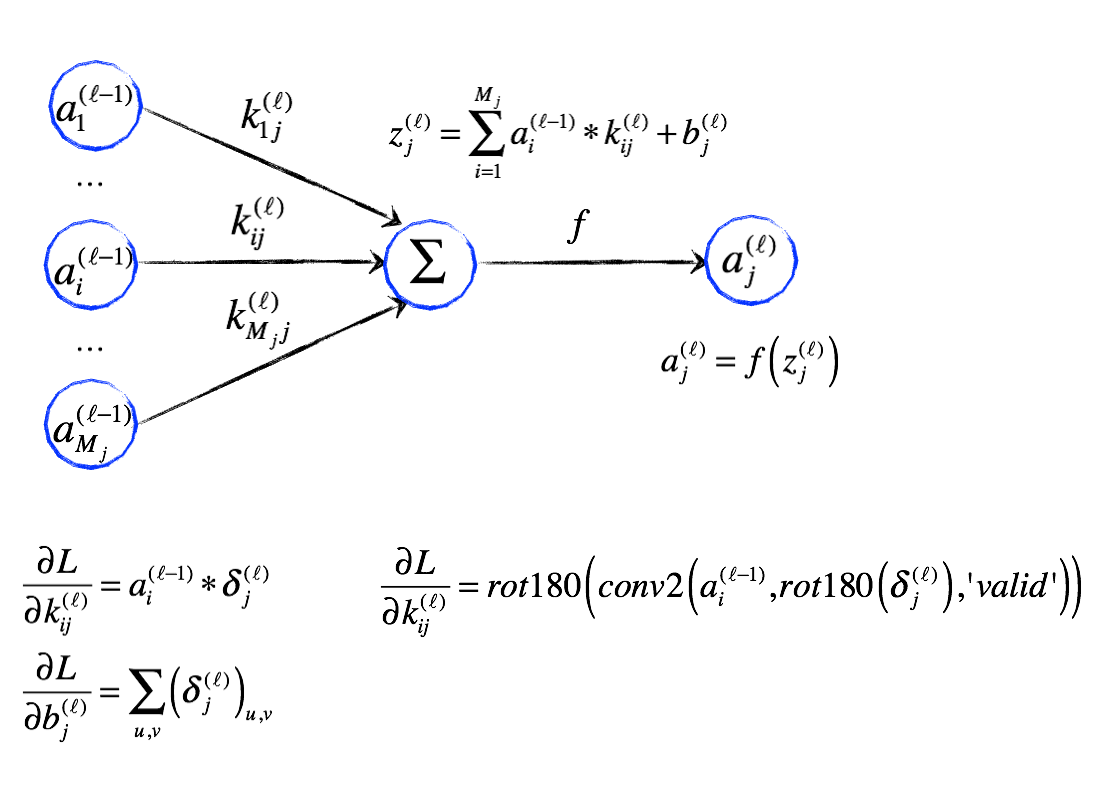
\includegraphics[width=0.85\textwidth]{conv-fprog-1.png}
  \end{figure}
\end{frame}

\begin{frame}[fragile]{反向传播:下采样}
  \begin{figure}
    \centering
    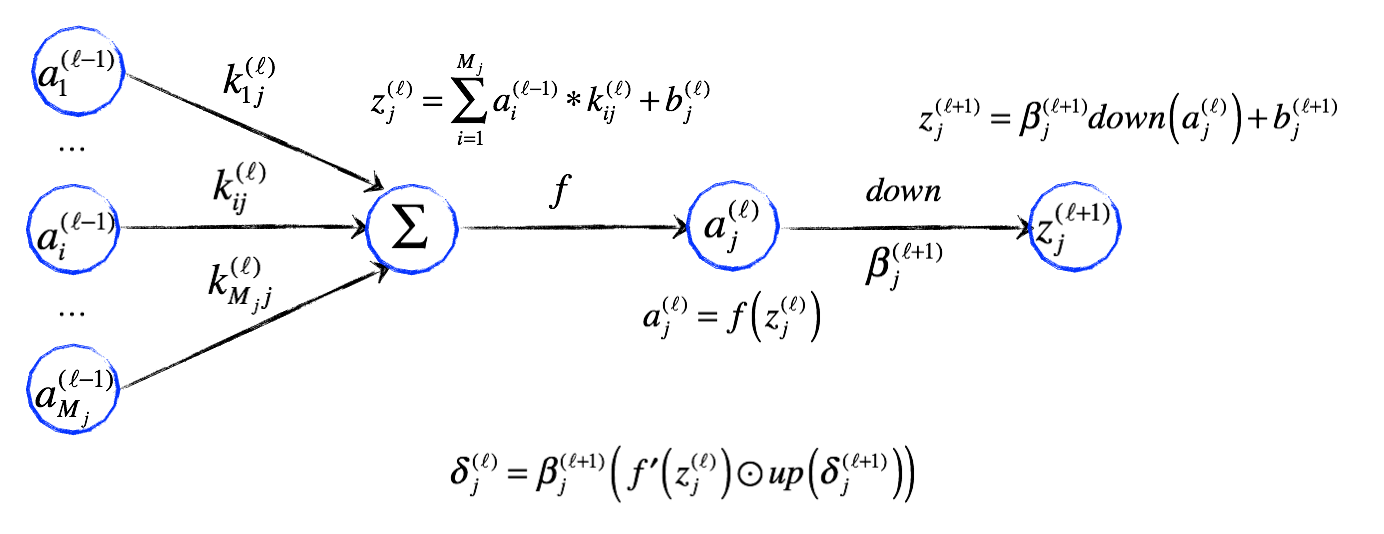
\includegraphics[width=1.0\textwidth]{conv-bprog-1.png}
  \end{figure}
\end{frame}

\begin{frame}[fragile]{前向计算:下采样}
  \begin{figure}
    \centering
    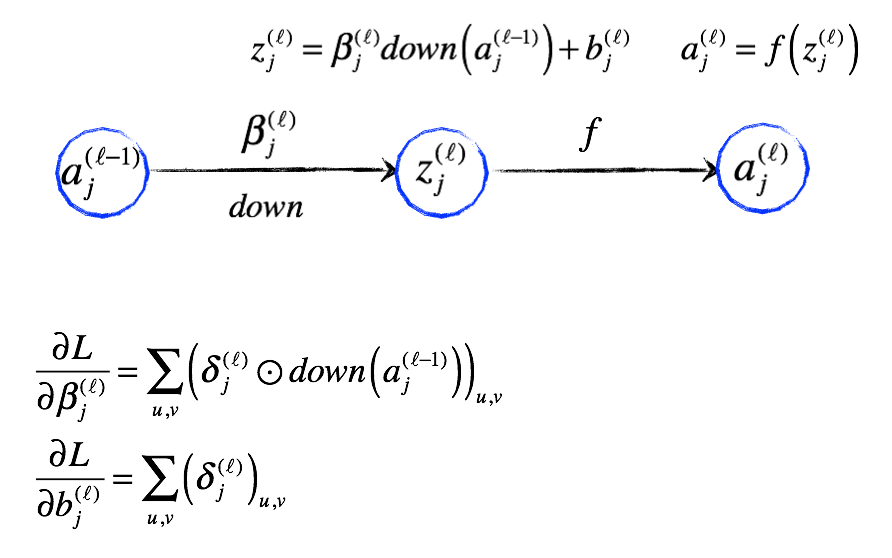
\includegraphics[width=0.8\textwidth]{conv-fprog-2.png}
  \end{figure}
\end{frame}

\begin{frame}[fragile]{反向传播:卷积}
  \begin{figure}
    \centering
    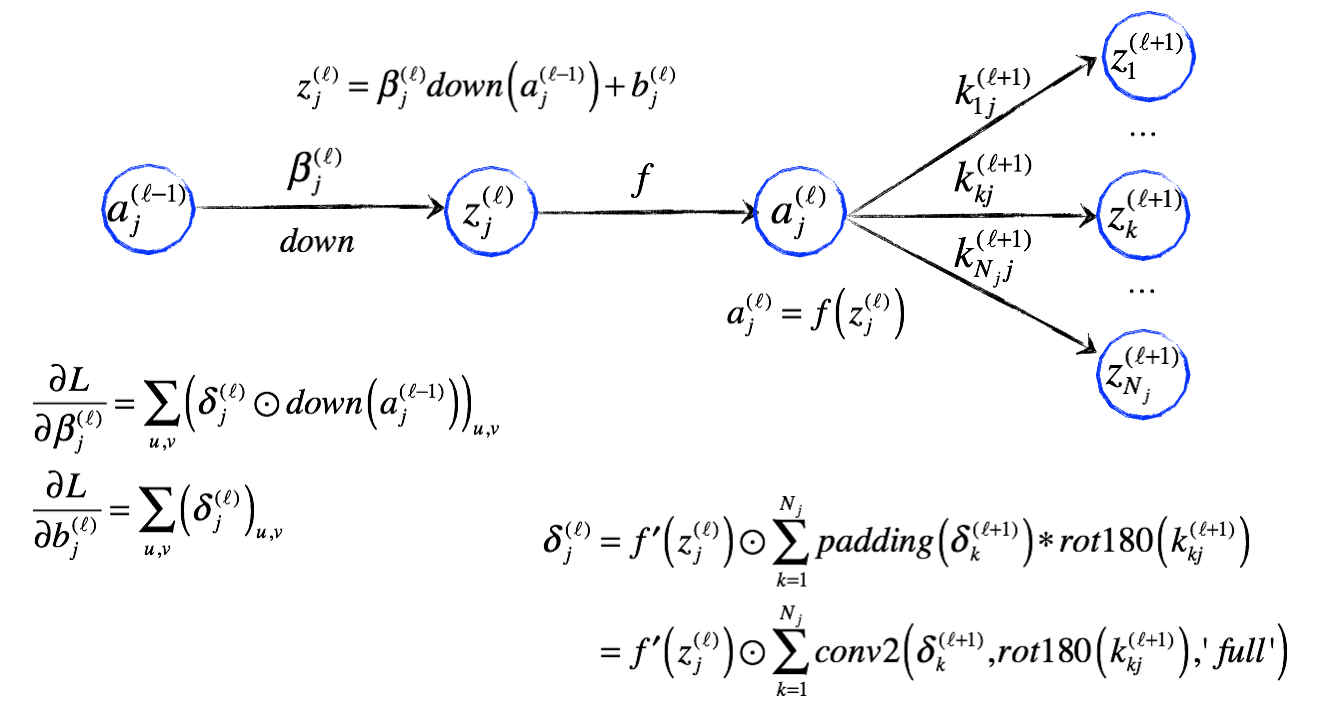
\includegraphics[width=1.0\textwidth]{conv-bprog-2.png}
  \end{figure}
\end{frame}
